% Modified version of computer science mindmap
% see: http://www.texample.net/tikz/examples/computer-science-mindmap/, respectively
% from the PGF/TikZ manual (Author is Till Tantau)
% There is a simple solution for coloring inter child connections correctly
% when using circle connection bars. It is actually in the manual but not directly visible.

\documentclass{standalone}

\usepackage{tikz}%
\usetikzlibrary{mindmap,trees}%
\usetikzlibrary{backgrounds}%

% This is a list of eight colors that are distinguishable for people with 
% every type of color vision deficiency (often misleadingly called colorblindness).
% see https://jfly.iam.u-tokyo.ac.jp/color/ for more information.
\definecolor{cb-darkgrey}{RGB}      { 50,  50,  50}% darkgrey
\definecolor{cb-blue}{RGB}          {  0, 114, 178}% blue
\definecolor{cb-orange}{RGB}        {230, 159,   0}% orange
\definecolor{cb-bluishgreen}{RGB}   {  0, 158, 115}% bluishgreen
\definecolor{cb-vermillion}{RGB}    {213,  94,   0}% vermillion
\definecolor{cb-skyblue}{RGB}       { 86, 180, 233}% skyblue
\definecolor{cb-reddishpurple}{RGB} {204, 121, 167}% reddishpurple
\definecolor{cb-yellow}{RGB}        {240, 228,  66}% yellow

\begin{document}

\centering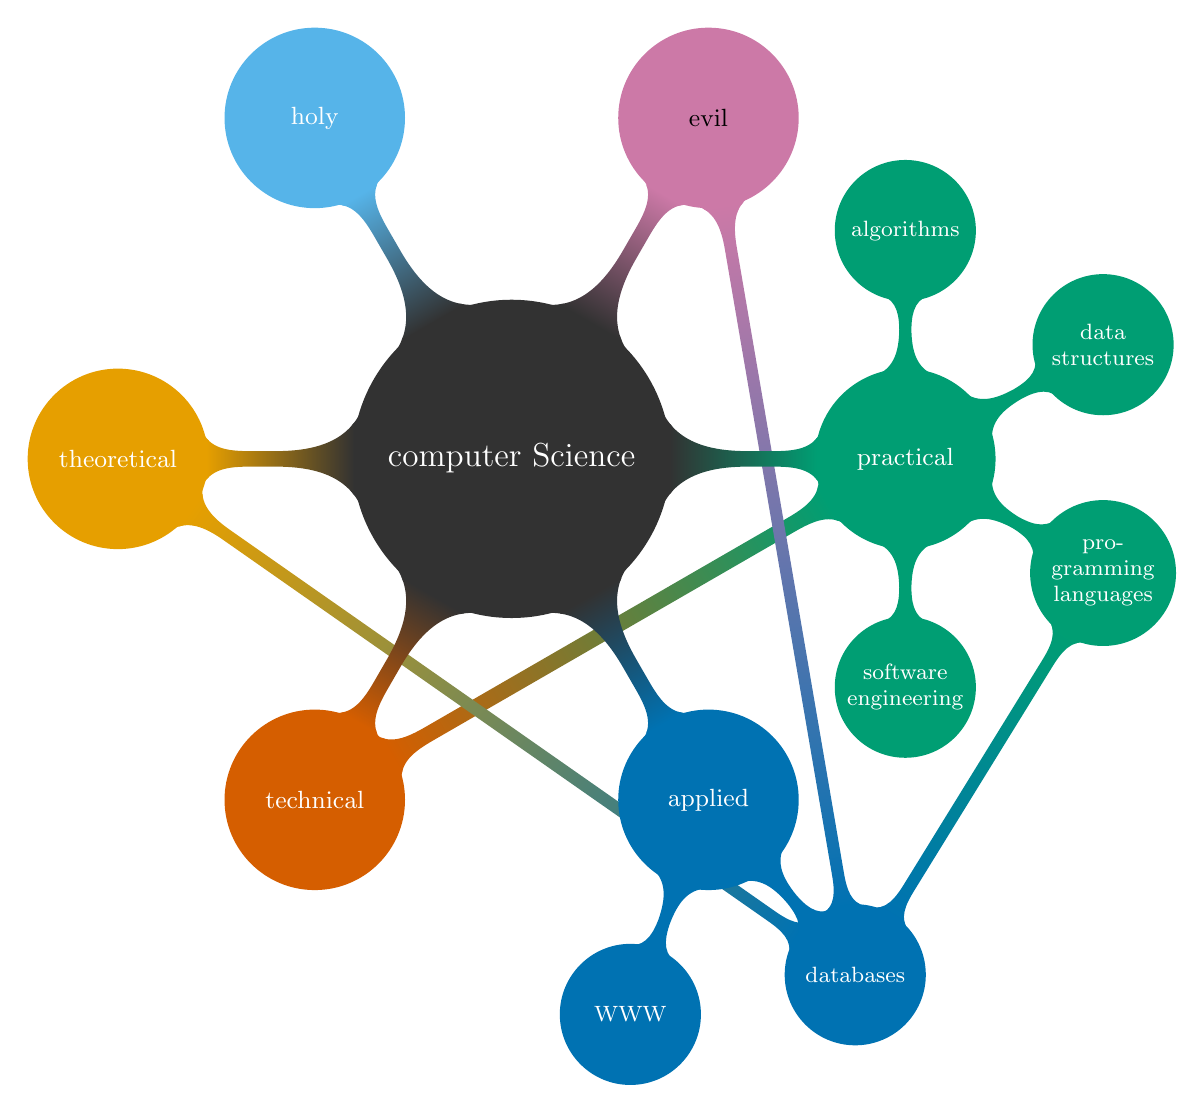
\begin{tikzpicture}[mindmap]
% DO NOT USE LINE BREAKS WITHIN THE PATH!
\path[mindmap, concept color=cb-darkgrey,text=white]
	node[concept] {computer Science}
	[clockwise from=0]
		child[concept color=cb-bluishgreen] {
			node[concept] (pr) {practical}
			[clockwise from=90]
				child { node[concept] (algo) {algorithms} }
				child { node[concept] {data structures} }
				child { node[concept] (pl) {pro\-gramming languages} }
				child { node[concept] (se) {software engineer\-ing} }
		}
		child[concept color=cb-blue] {
			node[concept] {applied}
			[clockwise from=-50]
				child { node[concept] (db) {databases} }
				child { node[concept] {WWW} }
		}
		child[concept color = cb-vermillion] {
			node[concept] (tc) {technical}
		}
		child[concept color = cb-orange] {
			node[concept] (theo) {theoretical}
		}
		child[concept color = cb-skyblue] {
			node[concept] {holy}
		}
		child[concept color = cb-reddishpurple, text=black] {
			node[concept] (evil) {evil} 
		}
;

	\begin{pgfonlayer}{background}
		\path (pr) to[circle connection bar switch color = from (cb-bluishgreen) to (cb-vermillion)] (tc);
		\path (db) to[circle connection bar switch color = from (cb-blue) to (cb-orange)] (theo);
		\path (pl) to[circle connection bar switch color = from (cb-bluishgreen) to (cb-blue)] (db);
		\path (db) to[circle connection bar switch color = from (cb-blue) to (cb-reddishpurple)] (evil);
	\end{pgfonlayer}

\end{tikzpicture}

\end{document}
